\documentclass[12pt]{article}

\usepackage[margin=1in]{geometry}
\usepackage{setspace}
\usepackage{csquotes}
\usepackage{graphicx}
\usepackage[version=4]{mhchem}
\usepackage{float}
\usepackage{textcomp}
\usepackage{subcaption}
\newcommand{\mnras}{MNRAS}
\newcommand{\apj}{ApJ}
\newcommand{\aap}{A\&A}
\usepackage[style=apa, backend=biber]{biblatex}
\addbibresource{references.bib}

\setstretch{1.5}

\begin{document}

\begin{titlepage}
    \centering
    \begin{figure}[htbp]
        \centering
        
\includegraphics[width=0.5\linewidth]{graphics/Title_page/swinburne_landscape_logo.png}
        \label{fig:placeholder}
    \end{figure}
    \vspace*{2cm}
    {\Large \textbf{Literature Review}}\\[1.5cm]
    {\large Riley Webster}\\[0.5cm]
    {\large Honours Project A}\\[0.5cm]
    {\large Semester 1, 2026}\\[2cm]
    \vfill
\end{titlepage}

\tableofcontents
\newpage

\section{Introduction} \label{sec: Introduction}
In astronomy, the group of objects that make up temporary phenomena such as supernovae (SNe), gamma ray bursts and tidal disruption events are known as transients. They are one of the most important phenomena to observe, as the data can lead to extraordinary discoveries such as the accelerating expansion of the Universe \parencite{riess_observational_1998, perlmutter_measurements_1999}. SNe are particularly important due to a specific type of supernova (SN) called type Ia Supernovae (SNe Ia). 

When SNe Ia are observed, their brightness can be plotted as a function of time. Following standardisation of the light curve, the light curves all reach a well known peak luminosity with some remaining scatter \parencite{martin_o_2024, kelsey_concerning_2022, ginolin_ztf_2025}. This peak luminosity can be used to then find the distance to the location of the detonation, using these distance calculations, the parameters that describe the properties of the Universe (\(\Omega_m, H_0, w, etc\)) can be determined. 

However, the current methods of standardisation show that systematic errors lie in the standardisation of these SNe. If these systematic errors can be accounted for, then truly representative light curves of these SNe can be used to produce more precise cosmological calculations. One of the methods to find new factors to account for in standardisation, is the study of host galaxy properties and their correlation with SNe Ia populations. If the light curves can be standardised based on factors that are intrinsic to the SNe Ia progenitor, then the better standardised the light curves can be which results in better determinations of \(\Omega_m, H_0, w, etc\).

\section{Supernova Ia physics and Progenitor Channels} \label{sec: Supernova Ia physics and Progenitor Channels}
\subsection{Standardisation} \label{subsec: Standardisation}
Type Ia Supernovae (SNe Ia) are standardisable candles, which means that upon observation of a SN Ia, the observed brightness follows a predictable evolution\parencite{martin_o_2024,rigault_strong_2020}. With corrections for the stretch and colour of the SN, the light curve can be standardised which corrects the observed light curve to find the intrinsic luminosity of the SNe Ia. The corrections for the light curves can be found in equation \ref{Eq: The Tripp equation} which accounts for the colour and stretch of the supernovae to determine the distance modulus (\(\mu_{obs}\)) \parencite{tripp_two-parameter_1998}. Using this distance modulus you can then derive distances to the Supernovae. 

\begin{equation}
    \mu_{obs} = m^*_B-M_B + \alpha x_1-\beta c
    \label{Eq: The Tripp equation}
\end{equation}

In equation \ref{Eq: The Tripp equation} the distance modulus is the difference between the apparent magnitude, \(m^*_B\), of the supernova and the absolute magnitude, \(M_B\) of the supernova. The remaining parameters are the stretch \(x_1\) and the colour \(c\) where \(\alpha\) and \(\beta\) are the stretch and colour coefficients where \(\alpha\) falls between 0.14 and 0.15 and \(\beta\) is between 2.9 and 3.5 \parencite{brout_pantheon_2022, martin_o_2024}. 

The stretch parameter is the parameter that corrects for the width of the light curve due to different distributions and masses of \ce{^{56}Ni} in the ejecta of the supernova \parencite{deckers_constraining_2022}. The colour is corrected due to the intrinsic components of the supernova and the surrounding environment such as dust, which can cause a redshift of the light, altering the shape of the light curve \parencite{kelsey_concerning_2022}. \(m^*_B\) is the apparent magnitude of the SNe Ia which is how bright the object appears from Earth and \(M_B\) is the absolute magnitude of the SNe Ia which is how bright the SNe Ia is from 10 parsecs away. 

Using the resulting \(\mu_{obs}\) from equation \ref{Eq: The Tripp equation}, you can acquire the luminosity distance \(d_L\) to the object using equation \ref{Eq: luminosity distance equation from distance modulus}, noting that the coefficient 10 is in units of parsecs \parencite{brout_pantheon_2022}. 

\begin{equation}
    d_L = 10 (10^{\mu/5})\
    \label{Eq: luminosity distance equation from distance modulus}
\end{equation}

From this equation, the luminosity distance can then be used to calculate cosmological parameters such as the density parameters for matter and radiation \(\Omega_m\) and \(\Omega_r\) and the equation of state parameter that describes how the density of matter, radiation and dark energy change in time \(w_{m}, w_{r}, w_{\Lambda}\) \parencite{brout_pantheon_2022}. Cosmological quantities are important, as they represent the contents of the Universe and thus be used to determine properties of the Universe. Standardisation of the supernovae and accounting for the different stretches and colours that are observed in the light curves results in more accurate distance calculations and better calculations of the cosmological parameters. 

The standardisation of SNe Ia light curves are not perfect, \textcite{brout_pantheon_2022,martin_o_2024,wiseman_further_2023,rigault_strong_2020} all show how the Tripp equation still leaves residual scatter of the distance modulus, which can be seen in Figure \ref{fig: Martin et al., 2024 Hubble Residuals as a function of galaxy stellar mass}. Research continues to determine how to improve standardisation methods that result in cosmological parameters that better represent the observed properties of the Universe. The Hubble residual is the measure of scatter in the calculation of the distance modulus, it's determined by the subtraction of the distance modulus calculated from a specific cosmology, \(\mu_{cos}\), from the result of equation \ref{Eq: The Tripp equation}, seen in equation \ref{Eq: Hubble residual equation}. It has been found that the scatter after corrections using the Tripp equation is reduced to 0.15 magnitude, leading to the conclusion that further corrections based on different properties are needed to standardise these light curves \parencite{brout_pantheon_2022,kelsey_concerning_2022, martin_o_2024}.

\begin{equation}
    \Delta\mu = \mu_{obs} - \mu_{cos}\
    \label{Eq: Hubble residual equation}
\end{equation}

\begin{figure}[htbp]
    \centering
    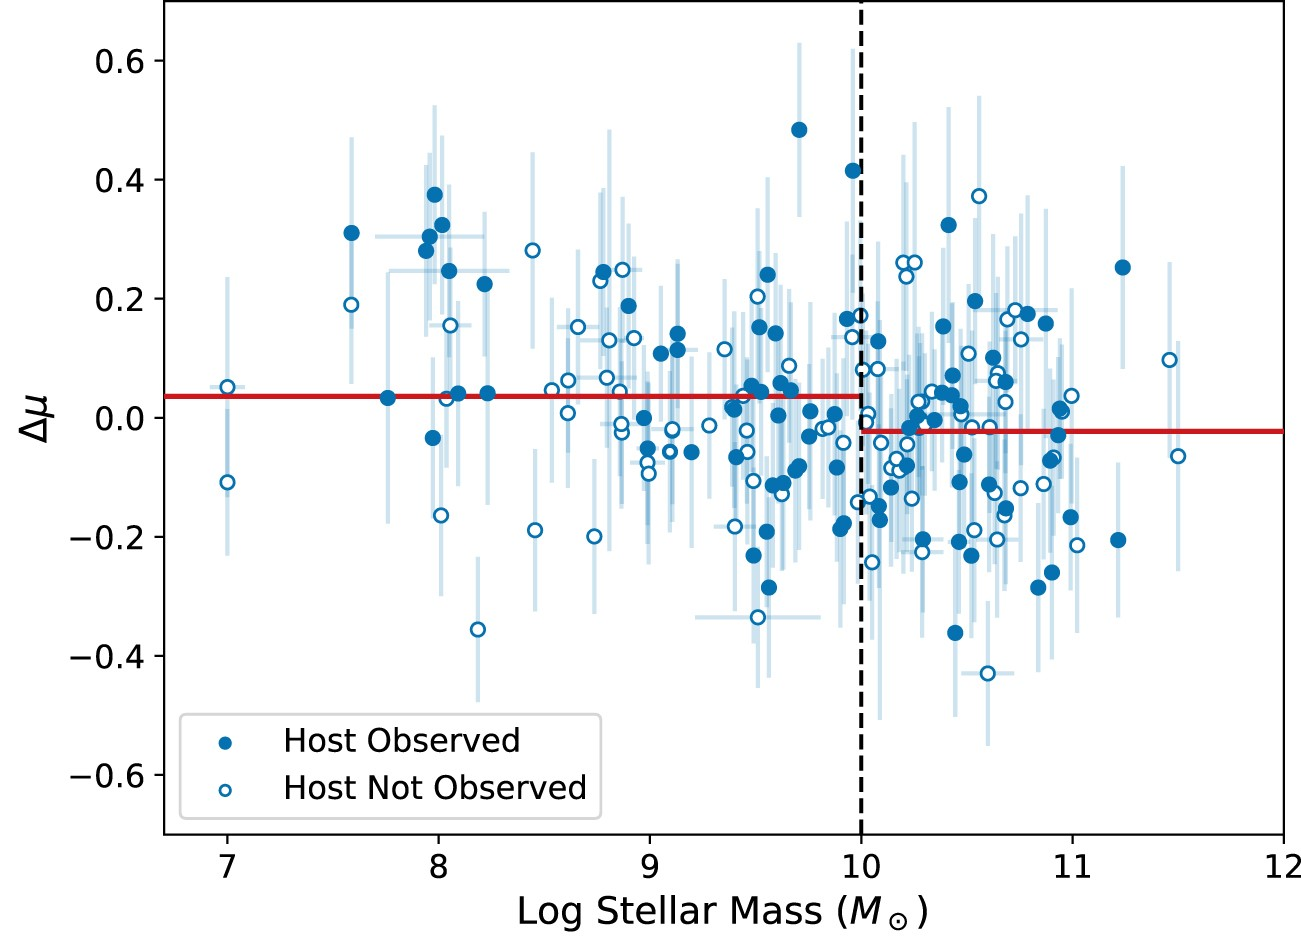
\includegraphics[width=0.8\linewidth]{graphics/SNIa_Physics_and_Progenitor_Channels/Hubble_residuals_Martin_2024.png}
    \caption{A figure taken from \textcite{martin_o_2024} that shows the scatter in Hubble residuals using 179 SNe Ia from the Foundation Survey dataset that is used in \textcite{martin_o_2024}'s analysis as a function of the host galaxy mass. The average Hubble residual is a step function at a host galaxy stellar mass of \(10\textup{M}_\odot\).}
    \label{fig: Martin et al., 2024 Hubble Residuals as a function of galaxy stellar mass}
\end{figure} 
    
A contentious correction that is made after the corrections made in equation \ref{Eq: The Tripp equation} to the SNe Ia light curves, is that of the host galaxy mass step\parencite{kelly_hubble_2010,sullivan_dependence_2010, lampeitl_effect_2010}. This remaining correlation showed that SNe Ia are 10 per cent brighter in more massive host galaxies, which lead to a noticeable difference in the equation of state parameter for dark energy (\(w_{\Lambda}\)). \textcite{kelly_hubble_2010}, who found that SNe Ia in more massive host galaxies were\(\simeq 0.1\) mag brighter than SNe Ia in less massive host galaxies, used 70 SNe Ia from the Sloan Digital Sky Survey with a redshift range \(0.015<z<0.08\) and determined that when using \(\mu_{obs}\) from 30 SNe Ia with host galaxies that have a stellar mass less than \(10^{10.8}\textup{M}_\odot\) the equation of state parameter is  \(w_{\Lambda} = -0.78^{+0.152}_{-0.108}\) whereas for 30 SNe Ia with host galaxies with a stellar mass greater than \(10^{10.8}\textup{M}_\odot\),\(w_{\Lambda} = -1.03^{+0.217}_{-0.143}\).

For the standard \(\Lambda\)CDM model of the Universe, the density of dark energy is taken as constant which implies an equation of state parameter \(w_{\Lambda}=-1\). And as can be seen in \textcite{kelly_hubble_2010}, using SNe Ia that are in less massive galaxies don't reflect the \(w=-1\) that is accepted in the modern model of the Universe. The error goes beyond the uncertainty of the determination of \(w_{\Lambda}\), showing that there is a systematic error in the standardisation of SNe Ia samples that are used in cosmology. This finding by \textcite{kelly_hubble_2010} was corroborated by \textcite{lampeitl_effect_2010} who used 361 SNe Ia from the SDSS-II Supernova Survey and limited the redshifts of the sample to \(z<0.21\). \textcite{lampeitl_effect_2010} found the more massive and lesser star formation rate (SFR) galaxies, hosted SNe Ia that were \(\simeq 0.1\) mag brighter than SNe Ia that were in galaxies of lower stellar masses. Finally, \textcite{sullivan_dependence_2010} using 195 SNe Ia from the Supernova Legacy Survey within redshift \(z <0.85\) also independently found that SNe Ia in higher mass host galaxies are 0.06–0.09 mag brighter than SNe Ia in galaxies with lower stellar mass. 

Although older, \textcite{kelly_hubble_2010,sullivan_dependence_2010, lampeitl_effect_2010} independently found the correlation of Hubble residuals with the stellar mass of the supernovas host galaxy and provided the initial mass step correction to further standardise supernova light curves. \textcite{kelly_hubble_2010,sullivan_dependence_2010, lampeitl_effect_2010} also demonstrates how the mass step is found across three different surveys and a redshift up to 0.85. Showing that the mass step correction is applicable systematically in the light curve measurements of SNe Ia used as standardisable candles in cosmology, although \textcite{kelly_hubble_2010,sullivan_dependence_2010, lampeitl_effect_2010} originally found and corrected for the mass step, the physical mechanics of why this difference in brightness is observed across more massive galaxies is not known. 

\subsection{Progenitor Channels} \label{subsec: Progenitor Channels}
It is accepted that the star that undergoes a supernova, producing the characteristic SNe Ia light curve is a carbon-oxygen (C-O) white dwarf \parencite{hoyle_nucleosynthesis_1960}. But white dwarfs don't undergo a supernova during their evolution, thus requiring other progenitor channels to be explored\parencite{antonini_evolution_2026}. The two popular progenitor channels for SNe Ia are the single degenerate scenario (SD) and the double degenerate scenario (DD). SD proposes that before an SN Ia event occurs, the system that was there before consisted of a C-O white dwarf that was accreting material from a non-degenerate companion star in a binary orbit\parencite{whelan_binaries_1973}. Whilst the DD scenario presents the idea of a merger between two degenerate stars such as two C-O white dwarfs and could also result in a supernova\parencite{iben_supernovae_1984}. 

The SD and DD progenitor models have been popular for decades and with recent research indicating that there is more nuance to these two progenitor channels that can cause the variety of the light curves observed by astronomers. \textcite{deckers_constraining_2022} study shows that out of 115 SNe Ia events that were detected by the Zwicky Transient Facility (ZTF), 67 per cent of the observed supernova light curves could effectively be recreated by the TURTLS model where the luminosity of the explosions are a direct result of Chandrasekhar-mass explosions with extended distributions and masses of 0.4 to 0.6 \(\textup{M}_\odot\) of \ce{^{56}Ni}. \textcite{deckers_constraining_2022} shows that over two thirds of SNe Ia could be resulting from Chandrasekhar mass C-O white dwarf explosions, whilst also demonstrating that 11 per cent of the SNe Ia light curves in the sample aren't reproduced from Chandrasekhar mass explosions and 19 per cent of the sample cannot be constrained using the varied masses and distributions of \ce{^{56}Ni}.   

\textcite{deckers_constraining_2022} also demonstrates a method to determine flux excesses in six light curves of the SNe Ia in the sample, \textcite{deckers_constraining_2022} finds that these flux excesses are generally well produced by the non degenerate companion interaction models as well as the \ce{^{56}Ni} clumping models that also produced the light curves of the 67 per cent of the SNe Ia. Due to the limited sample size \textcite{deckers_constraining_2022} concludes that SNe Ia likely have numerous pathways to explosion hence the varied observed light curves, but it appears that those 67 per cent can be modelled through the SD scenario. \textcite{deckers_constraining_2022} urges more high cadence UV and NUV surveys with spectroscopic follow up be done to conclude with more confidence the explosion scenario of SNe Ia. 

In a similar vein to \textcite{deckers_constraining_2022}, \textcite{burke_early_2022} shows that using a model that used a template light curve of a SN Ia from SiFTO with a companion shock-heating component component on a sample of nine SNe Ia that have light curve data 16 days before the epoch of peak flux, are well fit by non-degenerate companion interaction with the ejecta. These fits support the SD scenario interpretation. \textcite{burke_early_2022} suggests that the ejecta from the mass accreting white dwarf, shock heats the surface of the non-degenerate companion star which produces the flux excess in the light curves. This corroborates with the findings of the six early excess (EEx) SNe Ia in \textcite{deckers_constraining_2022} which reported non-degenerate companion interactions effectively modelled the observed light curves. 

Interestingly \textcite{burke_early_2022} also reported that eight of the nine SNe Ia were near-UV to Blue in colour (i.e. SNe Ia that have negative colour parameter $c$), although \textcite{deckers_constraining_2022} only reports three of the six having blue colour whilst the other three were red colour. This observed difference in colour is not reconciled through cross examination of either study. Both studies are still limited to small sample sizes which makes it difficult to make broader conclusions about the cause of the flux excesses and thus difficult to constrain the possible progenitor channels for these SNe Ia. Both papers conclude that high cadence near-UV surveys that detect more SNe Ia early on will help in our understanding of these flux excesses in the light curves. 

Although light curve fitting and modelling has shown results in determining the possible progenitors systems of SNe Ia, there have been numerous studies on the correlations of SNe Ia light and the Host galaxy properties. \textcite{kelsey_concerning_2022} finds through the analysis of 675 photometrically classified SNe Ia from the Dark Energy Survey 5-year sample, that blue SNe Ia are found in host galaxies that have lower stellar mass with higher star formation rates and are more blue in colour. \textcite{kelsey_concerning_2022} makes the argument that the stars in these hosts are younger populations that are producing the more blue colours. 

Although an older study, \textcite{anderson_environments_2015} finds a similar trend with SNe Ia light tracing out the blue light from host galaxies using pixel statistics method. \textcite{anderson_environments_2015} asserts that because the light from SNe Ia traces out the bluer region of host galaxies with lower SFR that progenitors systems that are less than 100 Myr old are extremely rare or do not exist. \textcite{kelsey_concerning_2022} also finds this 'colour gradient' where star formation begins closer to the centre of the host galaxy and eventually spreading to the outskirts of the host. But \textcite{anderson_environments_2015} using the pixel method found that the more 'local' lower star formation rates host the bluer SNe Ia, leading to older progenitor systems producing SNe Ia. \textcite{kelsey_concerning_2022} finds that the colour of the SNe Ia as a function of the local host galaxy colour is more blue in more locally bluer host environments, both these findings would suggest that the progenitor systems of SNe Ia are old and happening in bluer environments.   

\subsection{Early Flux Excess} \label{subsec: Early Flux Excess}
Early flux excess in the light curves of SNe Ia are seen as bumps in the light curve before the flux of the SNe Ia has reached its peak. In 2012 a SN Ia was observed and the analysis of the light curve by \textcite{marion_sn2012cg_2016} showed an EEx flux in the V, B and U band photometry. This was the first analysis of a 'normal' SNe Ia that had an EEx flux and the conclusion drawn was that the progenitor system likely was a non-degenerate companion, that was shock heated and was lucky enough to have the right viewing angle so that the excess could be observed. 

\textcite{burke_early_2022} uses data which was obtained from high cadence follow up observations using Las Cumbres Observatory and Swift, found 9 SNe Ia that had good early light curve data. \textcite{burke_early_2022} found that the light curves were best explained via the shock heating of a non-degenerate companion where a C-O white dwarf was accreting mass from this companion and upon explosion, had ejecta interactions with the companion that results in the companion, at the right angle, emitting a near-U-V blue excess. This again corroborates with the discovery \textcite{marion_sn2012cg_2016} proposes that companion interactions with a non-degenerate star is the physical cause of the EEx observed.

Referring back to \textcite{deckers_constraining_2022} who had a sample size of 6 EEx SNe Ia, found that the EEx colour and the lifetime of the flux excess is consistent with their modelling of both companion and circumstellar medium (CSM) interaction as well as \ce{^{56}Ni} clumping in the outer ejecta of the white dwarf. \textcite{deckers_constraining_2022} argues that the EEx flux in SNe Ia is heterogeneous and can be caused by multiple different progenitors. \textcite{deckers_constraining_2022} is to contrast the previous studies as they conclude, that to be more definitive regarding the mechanisms behind the EEx in flux, one day cadence surveys will enable fast spectroscopic follow up which will grant the ability to make more confident conclusions about the physics of the EEx.

\textcite{lim_early_2023} is a case study on SN 2021hpr which exhibits the EEx in it's flux, similar to \textcite{marion_sn2012cg_2016} and \textcite{burke_early_2022}, the shock heating emission of the companion star for the white dwarf most suitably models the light curves of SN 2021hpr across the B, V, R and I bands from the Intensive Monitoring of Nearby Galaxies Survey which can be seen in Figure \ref{fig: Lim et al., 2023 the light curve of SN2021hyp}. Although the light curve fit well with a non degenerate companion model, \textcite{lim_early_2023} could not find evidence of any stripped mass of the companion that would've been expected following the explosion of the companion using spectroscopic follow-up. \textcite{lim_early_2023} also acknowledge that they did not assess the viability of other models that could cause the excess, such as a double detonation model or disk originated matter models.

\begin{figure}[htbp]
    \centering
    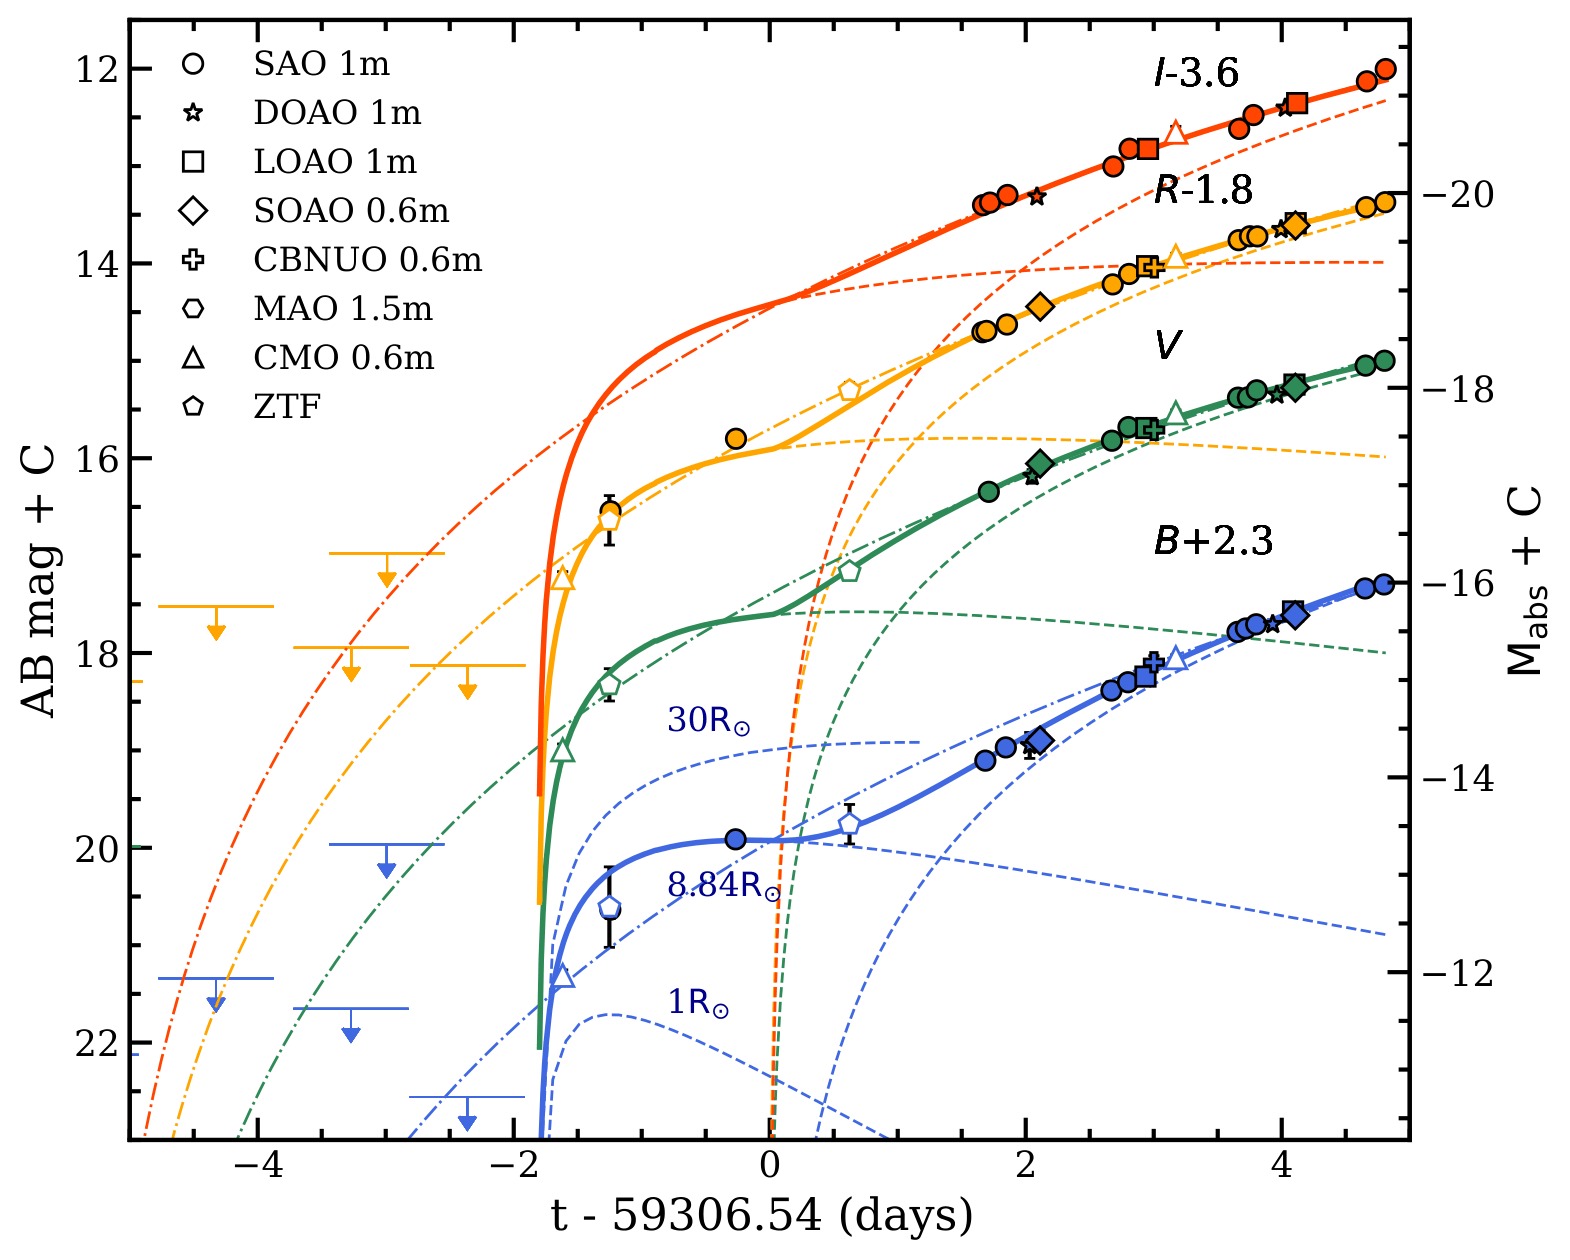
\includegraphics[width=0.8\linewidth]{graphics/SNIa_Physics_and_Progenitor_Channels/lim_2021_hpr_supernova_lightcurve.png}
    \caption{The light curves of SN2021hpr in magnitude space taken from \textcite{lim_early_2023}. The points are the observations, the dashed-dotted line is the light curve modelled by the simple power law model and the dashed lines are modelled light curves from \textcite{kasen_seeing_2010} which include the emission of light from the shock heating of a companion star. Finally, the solid lines are the two models combined and can be seen to line up well with the observations.}
    \label{fig: Lim et al., 2023 the light curve of SN2021hyp}
\end{figure}
 
 \textcite{lim_early_2023} shows that the light curve deviates from a simple power law model as well as the companion model from \textcite{kasen_seeing_2010} and has a bump across all bands which can be seen in Figure \ref{fig: Lim et al., 2023 the light curve of SN2021hyp}. But the combination of both the power law and the \textcite{kasen_seeing_2010} companion models produce a curve that fits the observations. 

The method used to detect the EEx fluxes in the SNe Ia data can vary, in \textcite{deckers_constraining_2022} they use the residuals in the light curves that are found by subtracting the modelled light curve generated using the TURTLS model from the observed light curve. If a positive residual is found in the light curve within the calculated 6 days after the explosion epoch \textcite{deckers_constraining_2022} classify that SNe Ia light curve as an EEx SNe Ia. 

In \textcite{burke_early_2022} the EEx flux SNe Ia are identified in a similar way to what was done in \textcite{lim_early_2023}, as \textcite{burke_early_2022} uses the same companion shock cooling models present in \textcite{lim_early_2023} from \textcite{kasen_seeing_2010}. \textcite{burke_early_2022} stipulates that they classify SNe Ia as EEx SNe Ia if there is data available within five days of the first detection, the best fit viewing angle is less than 90 degrees and the residuals in the g band show a systematic decreasing from the earliest epochs to then matching the modelled light curve. Finally in \textcite{marion_sn2012cg_2016} the EEx flux SNe Ia was detected through the comparison of the observed light curve to the fitted power model light curve where the observed data had to be three times the measurement uncertainty. 

\section{Host Galaxy Environment and SN Ia diversity} \label{sec: Host Galaxy Environment and SN Ia diversity}
\subsection{Host Galaxy Properties} \label{subsec: Host Galaxy Properties}
In section \ref{subsec: Progenitor Channels} it's clear that the environment of the SNe plays a factor in the shape of the light curve observed from an SN. Thus the properties of the host galaxies of SNe have been studied to determine the correlations between those properties and the locations of where SNe happen. \textcite{toy_reduction_2025} uses a sample of 1533 SNe Ia from the 'five-year' sample from the DES SN program. \textcite{toy_reduction_2025} using the Directional Light Radius method (DLR) to associate SNe Ia with a host galaxy and find that there is no step-like change in the Hubble residuals average across a normalised DLR, \(d_{DLR}\), of 1. But when splitting the sample to 'inner regions' where \(d_{DLR} < 1\) the Hubble residuals have a step in the averages of \(0.100 \pm 0.014\) mag when split across the host galaxies with a stellar mass of 10. But in the outer regions (\(d_{DLR}>1\)) \textcite{toy_reduction_2025} finds that the step in the Hubble residuals when split by host's with stellar masses of 10 is \(0.036\pm0.018\). \textcite{toy_reduction_2025} makes the conclusion that SNe Ia in the outer regions are less affected by the global host galaxy properties, although \textcite{toy_reduction_2025} notes that the different mechanics that produce this result is still unknown.

\begin{figure}[htbp]
     \centering
     % Top Image
     \begin{subfigure}[b]{0.6\textwidth}
         \centering
         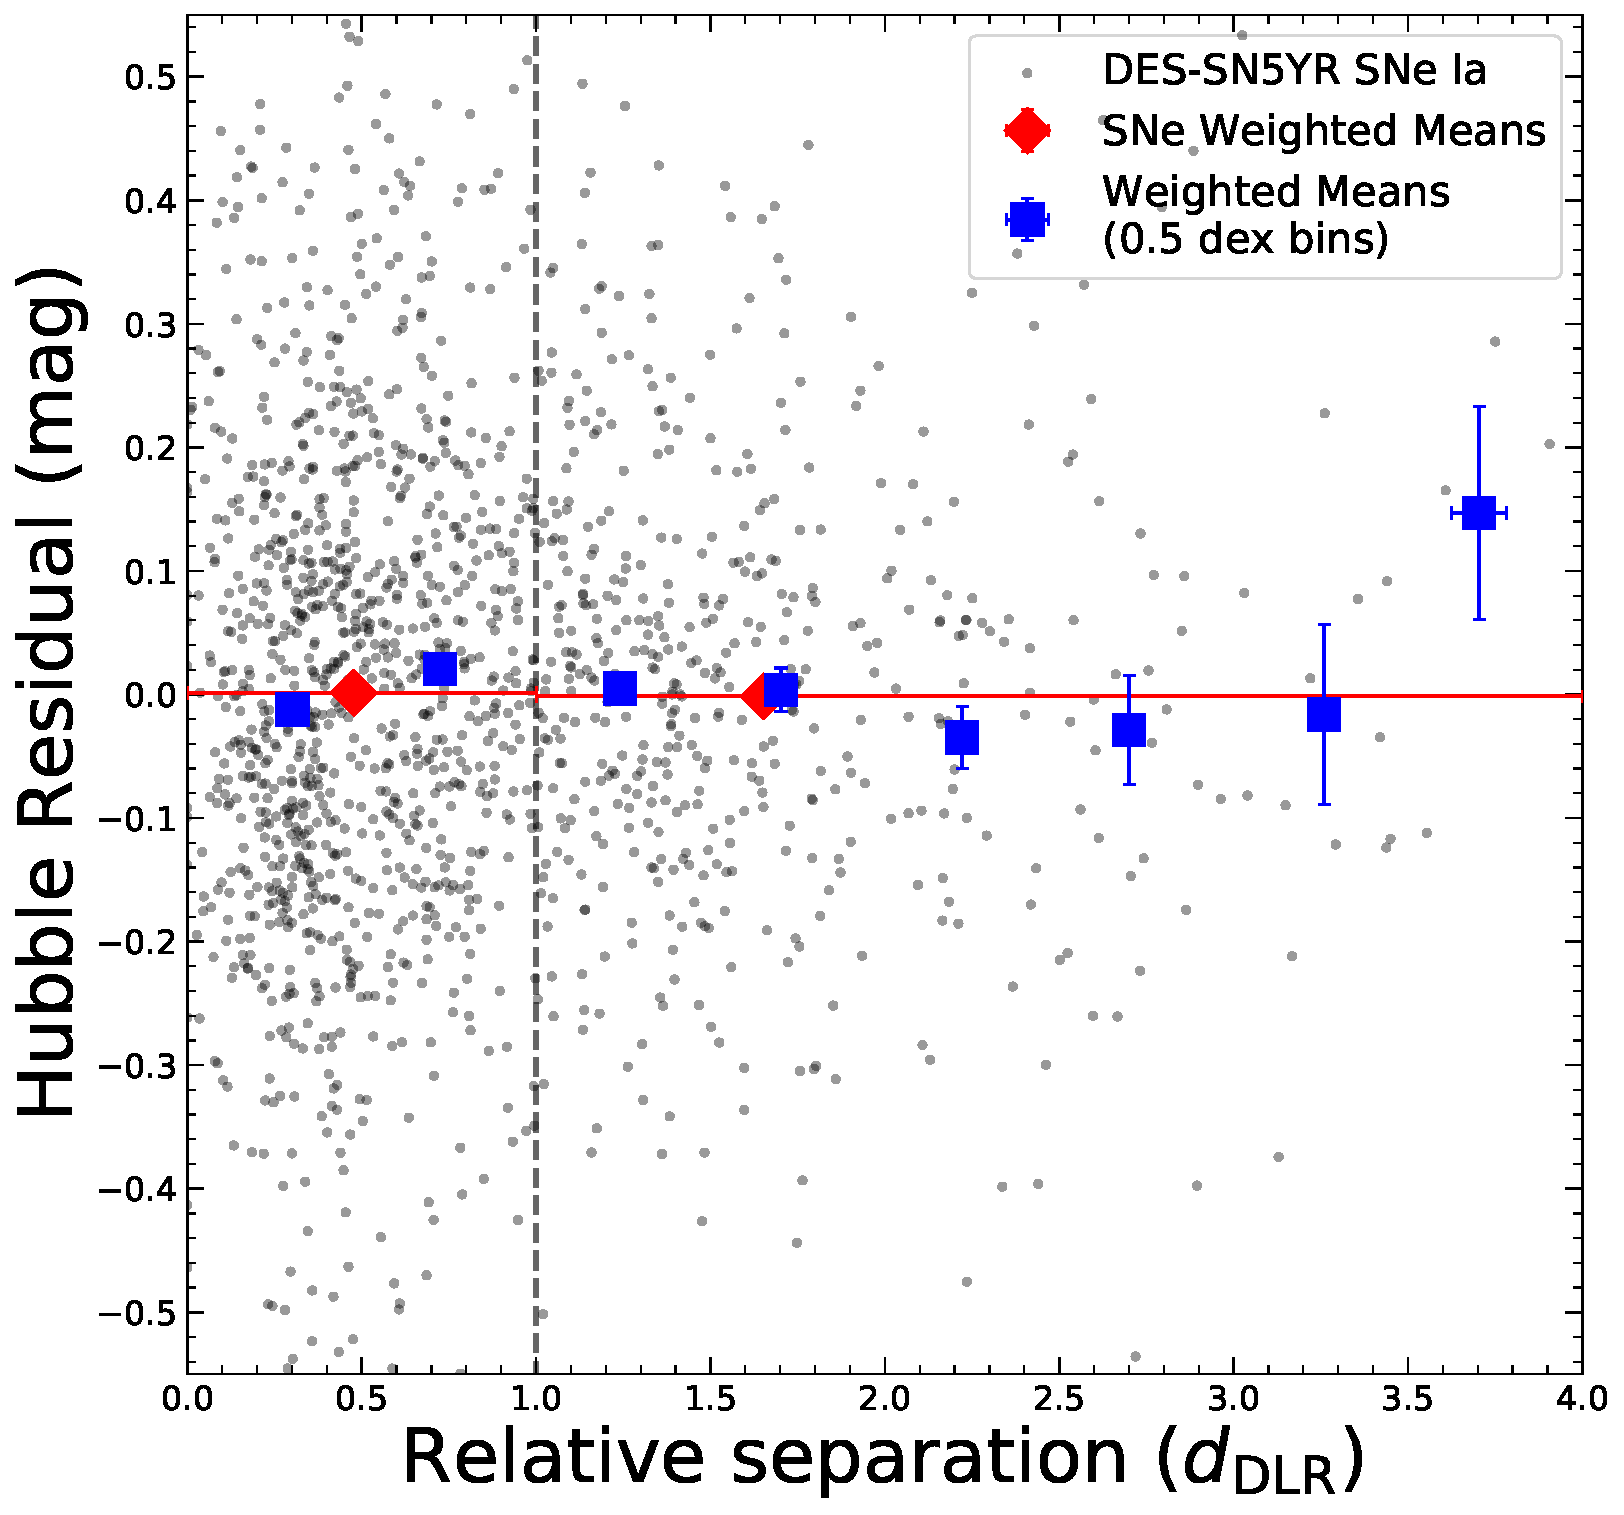
\includegraphics[width=\textwidth]{graphics/Host_galaxy_properties/muresvsddlr.pdf}
         \caption{}
     \end{subfigure}
     
     \vspace{1em} % Adds some vertical space between rows

     % Bottom Two
     \begin{subfigure}[b]{0.45\textwidth}
         \centering
         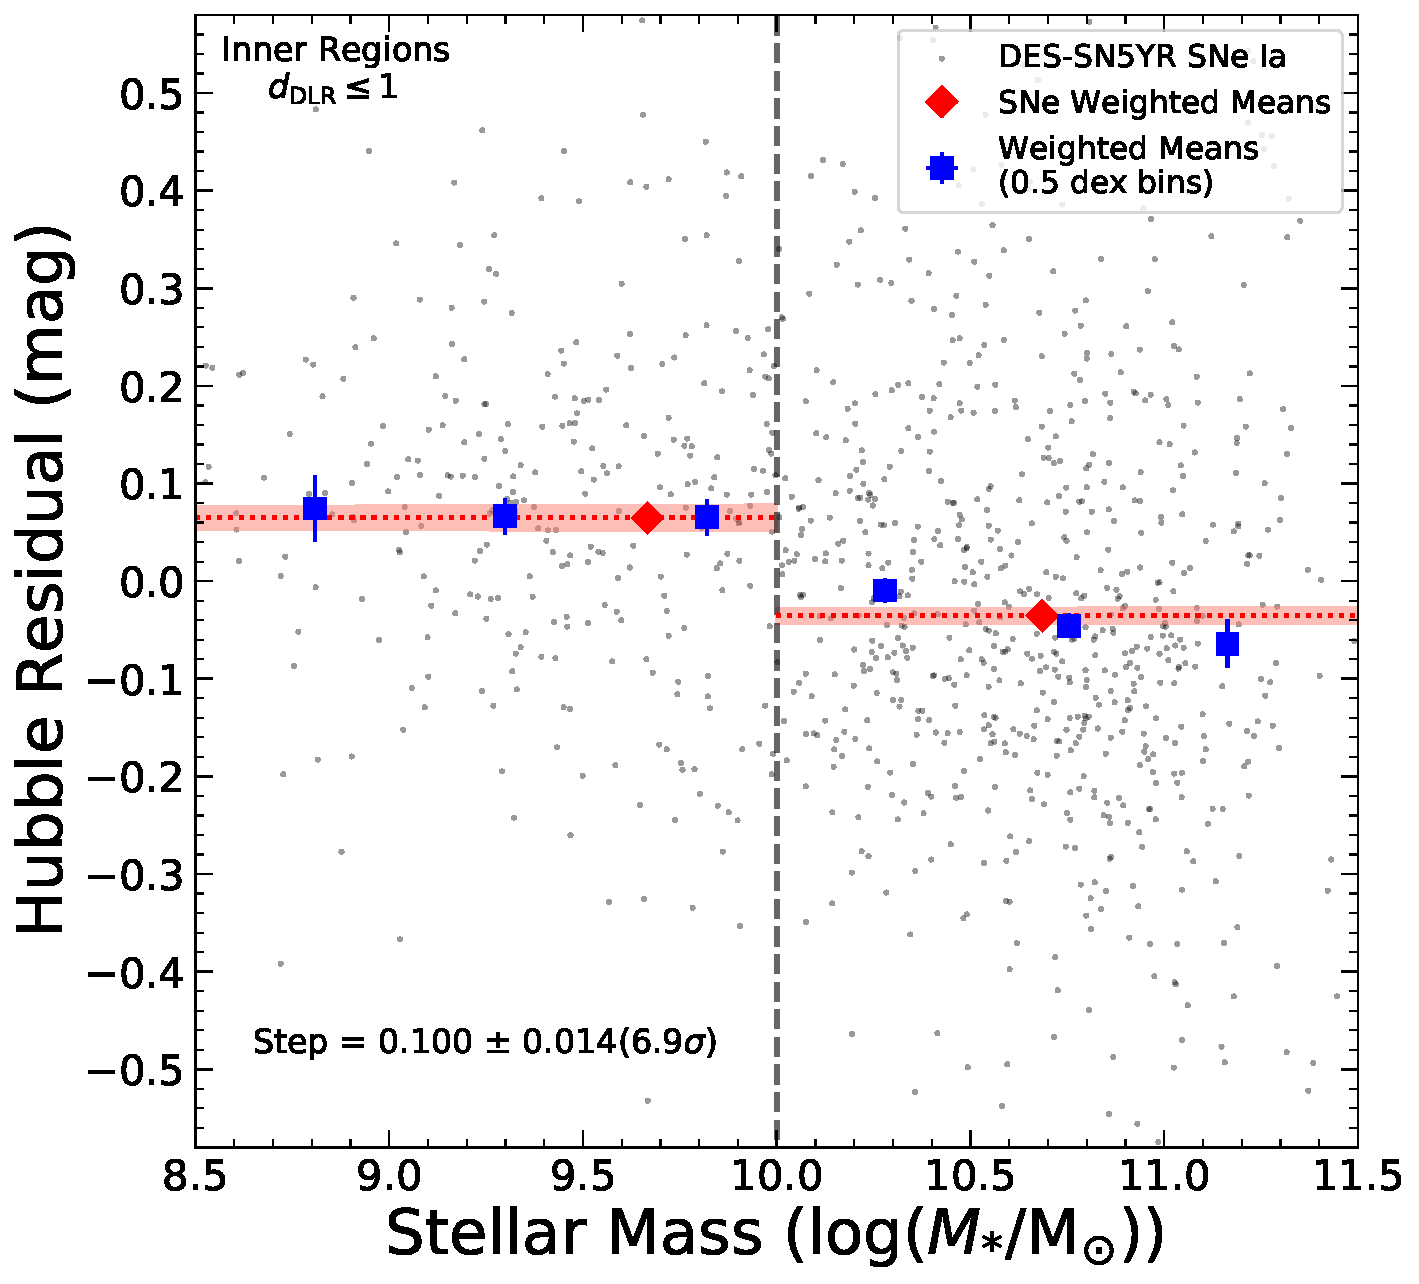
\includegraphics[width=\textwidth]{graphics/Host_galaxy_properties/innerregionsphilsample_extra_binshost_mass_step.pdf}
         \caption{}
     \end{subfigure}
     \hfill
     \begin{subfigure}[b]{0.45\textwidth}
         \centering
         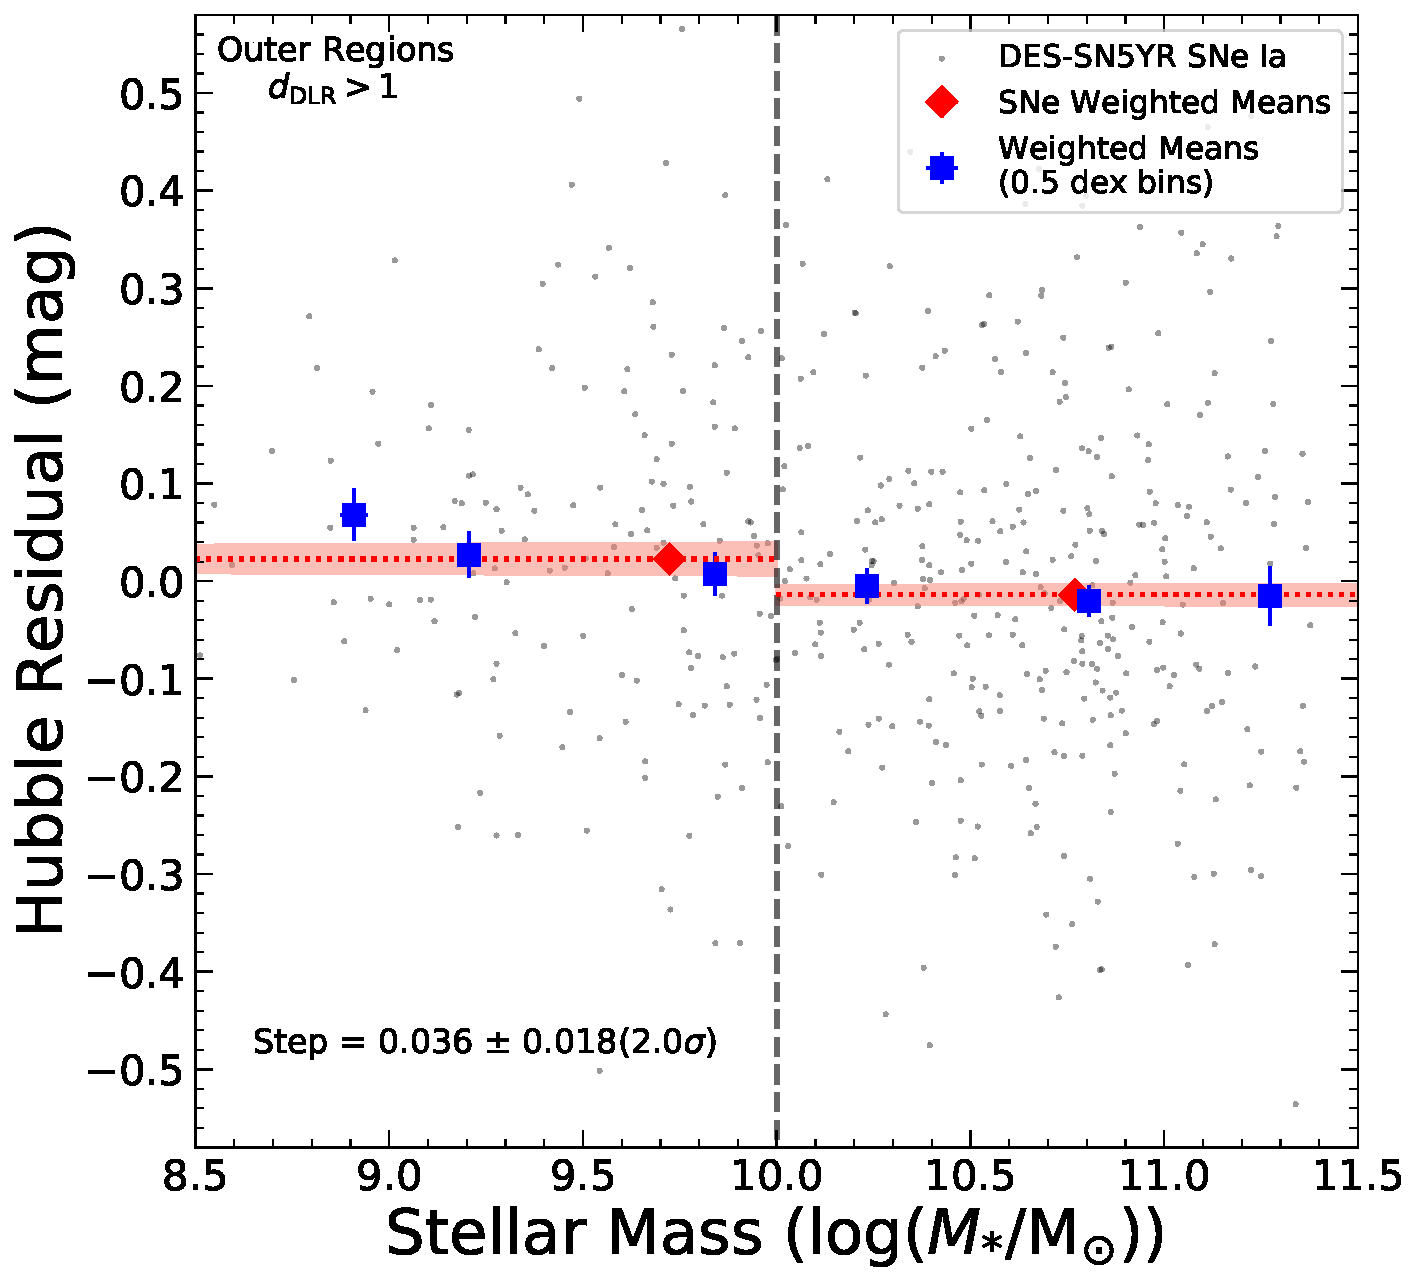
\includegraphics[width=\textwidth]{graphics/Host_galaxy_properties/outerregionsphilsample_extra_binshost_mass_step.pdf}
         \caption{}
     \end{subfigure}
     \caption{Taken from \textcite{toy_reduction_2025}, Figure (a) shows the mass step that can be seen in Figure \ref{fig: Martin et al., 2024 Hubble Residuals as a function of galaxy stellar mass} but as a function of the relative separation from the galaxy centre to the location of the SNe Ia. As a function of the relative separation, it's obvious that the step between Hubble residuals is greatly reduced. In images (b) and (c) which show the Hubble residuals for the inner regions and outer regions respectively, the mass step is found to be reduced for the SNe Ia in the outer regions of their host galaxies.}
     \label{fig: Figures of the mass step being reduced globally but being present within certain regions of the host, from the Marcus Toy paper.}
\end{figure}

By searching for these correlations with the host galaxy properties, an intrinsic property of the SNe Ia's environment could explain this observation of SNe Ia in higher mass galaxies being brighter than those in lower mass galaxies. As seen in \textcite{toy_reduction_2025}, the outer regions of the host galaxy appear to be less affected by whatever is changing the observed brightness of these SNe Ia. 

Another interesting property to study is the global colour of the Host galaxy, \textcite{kelsey_concerning_2022} finds that blue SNe Ia have higher homogeneity in the Hubble residuals. This higher homogeneity in blue SNe Ia was found across the global host galaxy mass, local host galaxy mass, global host galaxy colour and local host galaxy colour. \textcite{kelsey_concerning_2022} interprets this stronger homogeneity post-standardisation as a sign that the older, more globally red galaxies have had more time for SNe to occur and create dust that reddens the SNe Ia that happen afterwards, meaning that the red population is a heterogeneous one and could be made up of a different sub type of SNe Ia that needs to be standardised in a different way to reduce the step function in the residuals.

Another study, \textcite{ramaiya_dependence_2025}, finds correlations with SNe Ia and the stage of evolution that the host galaxy of the SNe Ia. \textcite{ramaiya_dependence_2025} uses 1685 SNe Ia from the DES SN sample and for the host galaxies \textcite{ramaiya_dependence_2025} uses a wide range of sources which include the Canada-France-Hawaii Telescope, the VLT Survey Telescope, the Subaru Hyper Suprime-Cam, the Visible and Infrared Survey Telescope for Astronomy and the Spitzer Space Telescope and the Herschel Space Observatory. This number of sources lets \textcite{ramaiya_dependence_2025} cover a wide range of light emitted from host galaxies for a robust study. As can be seen in Figure \ref{fig: Figure 8 from the Ramaiya et al., 2025 study showing the different colour corrections based on host galaxy stage of evolution.}, the colour nuisance parameter \(\beta\) changes based on the stage of evolution that the host galaxy is in. \textcite{ramaiya_dependence_2025} shows that the stage of the host galaxy's evolution which changes properties such as mass and SFR also affects the luminosities of the SNe Ia in their host galaxies.  

\begin{figure}[htbp]
    \centering
    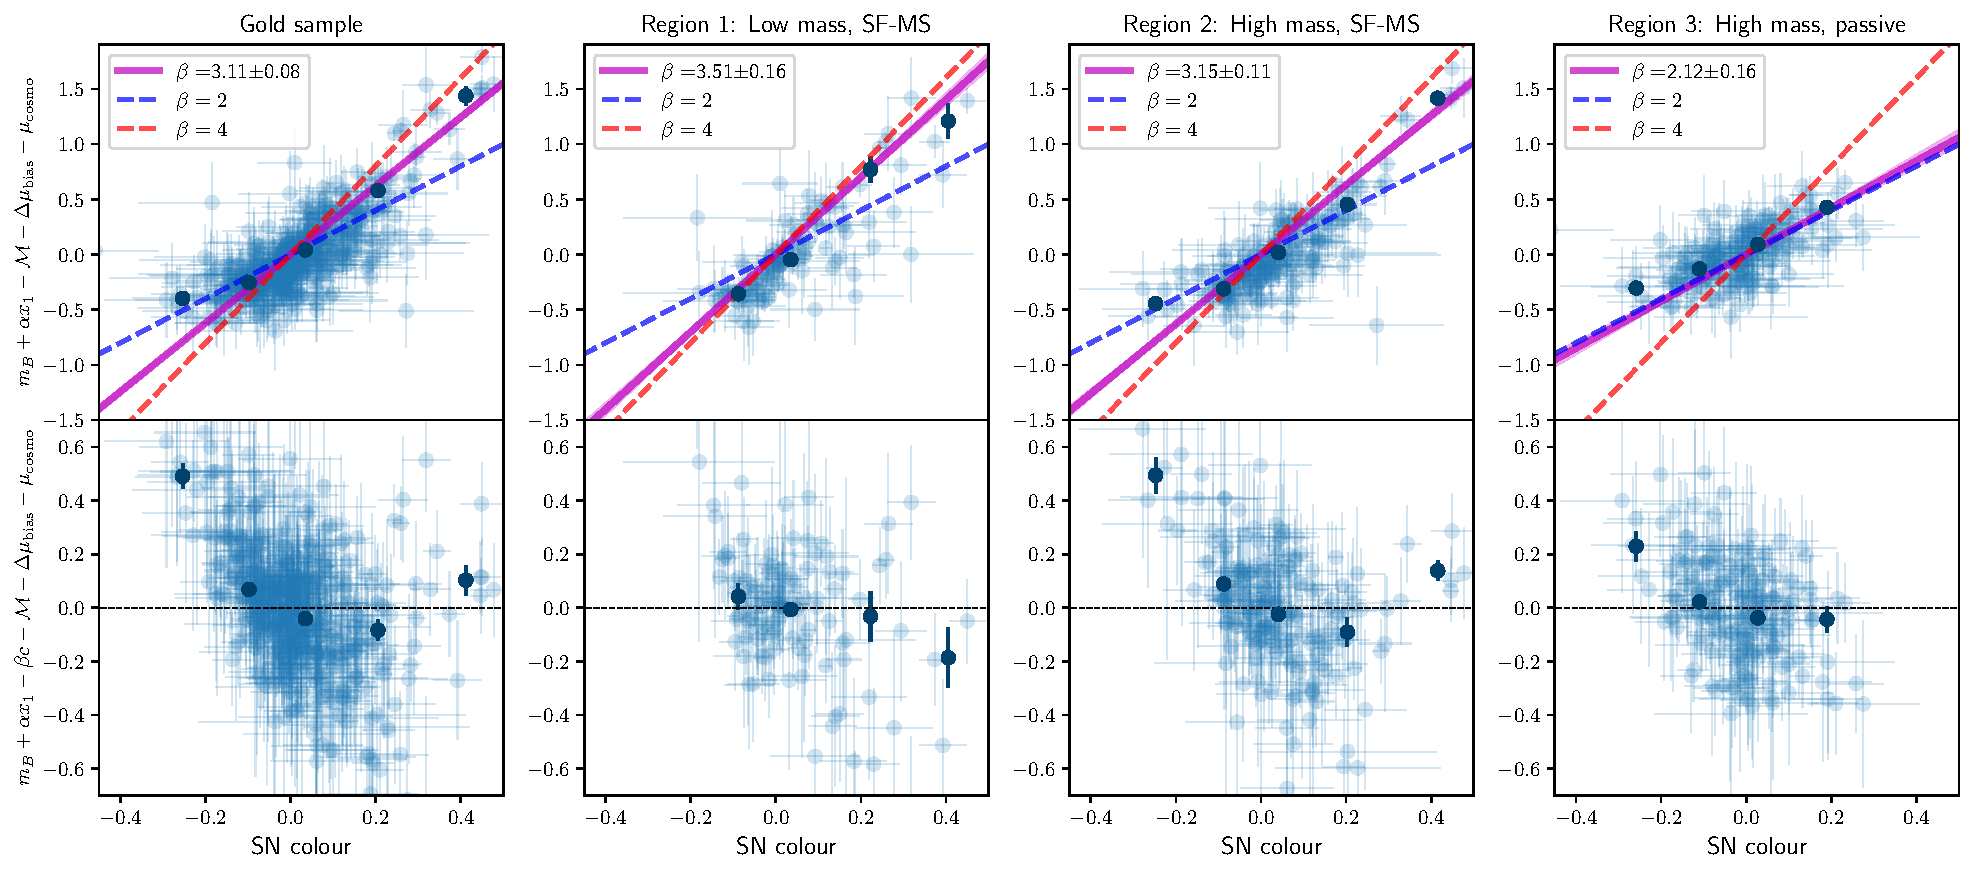
\includegraphics[width=\linewidth]{graphics/Host_galaxy_properties/betas_PLOT.pdf}
    \caption{Taken from \textcite{ramaiya_dependence_2025}, the plots on top are the Hubble residuals plotted as a function of SNe Ia colour, without the colour calibration term in the Tripp equation. The bottom plots show the Hubble residuals whilst correcting for colour as a function of the SNe Ia colour. The gold sample is the sample of all the SNe Ia from the DES SN sample, whilst the remaining three are the plots of the gold sample divided by the evolutionary stage the host galaxy is in.}
    \label{fig: Figure 8 from the Ramaiya et al., 2025 study showing the different colour corrections based on host galaxy stage of evolution.}
\end{figure}

Connecting both \textcite{ramaiya_dependence_2025} and \textcite{kelsey_concerning_2022} shows that the evolutionary stage of the host galaxy and ergo the age has an effect on the magnitudes of the SNe Ia. In \textcite{ramaiya_dependence_2025} \(\beta\) is noticeably different to the active star forming galaxies but once star formation ceases, the colour correction isn't as aggressive. \textcite{kelsey_concerning_2022} finds that hosts with a higher \(U - R\), which is a proxy for a younger star forming galaxy, finds that SNe Ia require a higher \(\beta\) which is also found in \textcite{ramaiya_dependence_2025}. The same relation for more blue galaxies, where \(U - R\) is lower requires smaller \(\beta\). This corroboration of an age-mass relation of host galaxies in \textcite{ramaiya_dependence_2025} and \textcite{kelsey_concerning_2022} shows that the age and evolutionary stage of the host must relate to the SNe Ia in a way that can reduce the scatter in the Hubble residuals.

\subsection{The Environment and Early Excess Flux} \label{subsec: The Environment and Early Excess Flux}
Host galaxy correlations are clearly important in the study of SNe Ia, as understanding the environment where SNe Ia are occurring in can help explain the physics of the SN. The correlations with host galaxy mass, DLR, colour and SFR have helped navigate what could be causing the remaining scatter in the Hubble residuals. But what correlations with host galaxy properties are there for EEx SNe Ia and could they help explain the additional bump in the light curve?   

Due to how small the samples sizes are for EEx SNe Ia, the studies of host galaxy properties correlating with properties of the EEx SNe Ia are limited. \textcite{deckers_constraining_2022} found, whilst acknowledging the small sample size doesn't allow them to make significant conclusions, that 5 of the 6 EEx SNe Ia have hosts with stellar masses lower then the mean of their sample \(<\log(\textup{M}_*/\textup{M}_{\odot})=9.82\). Because of the connection to lower mass hosts, \textcite{deckers_constraining_2022} postulates, stemming from \textcite{rigault_strong_2020} that the progenitor systems of EEx flux SNe Ia are likely to be from a younger population. 

A recent study by \textcite{wu_wfst_2026} uses a sample of 16 SNe Ia with data 16 days before the B band maximum light. \textcite{wu_wfst_2026} found 3 EEx Flux SNe Ia and could only associate two with a host galaxy, the conclusions are limited due to the limited data, regardless both the associated hosts of the 2 EEx SNe Ia had a lower stellar mass than the mean of the sample (\(\log(\textup{M}_*/\textup{M}_{\odot})=9.94\)). Whereas only one of the SNe Ia occurred in a host with a highest SFR of the sample (3.64\(\textup{M}_{\odot}yr^{-1}\)) whereas the second SNe Ia has the 4 lowest SFR of the sample. 

It is safe to say that without more detections of EEx SNe Ia, correlations with host galaxy properties will not be able to reach a sample size that allows for statistically significant analysis. This results in a lack of conclusions being able to be drawn about the niche phenomena observed in these light curves.

\section{Fink, Rubin and LSST} \label{sec: Fink, Rubin and LSST}
Over the course of this review it has become obvious that more and earlier data would provide the next steps for both progenitor channel and correlation constraining of SNe Ia with host properties. If more SNe Ia in hosts can be collected and much earlier before peak flux, then the correlations with host galaxy properties can be more easily studied which enables improvements for standardisation methods. 

The EEx SNe Ia are difficult to find, with most studies not being population studies but rather case studies, and the few population studies result in a sample size of 6 and 3 \parencite{deckers_constraining_2022, burke_early_2022, wu_wfst_2026}. The Vera C. Rubin Observatory which will be referred to as Rubin from here on out, is located in El Peñón peak of Cerro Pachón in Chile \parencite{bianco_optimization_2022}. The observatory hosts a 8.36 metre aperture and will have filters across a wavelength range of 320.5 nanometres to 1084.5 nanometres \parencite{bianco_optimization_2022}. The viewing cadence of LSST has an average revisit time of 3 days across the whole southern sky which, covers an area of 18000 $deg^2$ which gives the median number of revisits at 825 per site \parencite{bianco_optimization_2022, ivezic_lsst_2019}. As can be seen in Figure \ref{fig: Map of the fields that Rubin will visit with the median number of revists across different portions of the Southern Sky.} Some portions of the Southern Sky will be visited more than others but the main Wide-Fast-Deep (WFD) survey will have an average of 900 revisits across the 10 years that LSST will operate over.   

\begin{figure}[htbp]
    \centering
    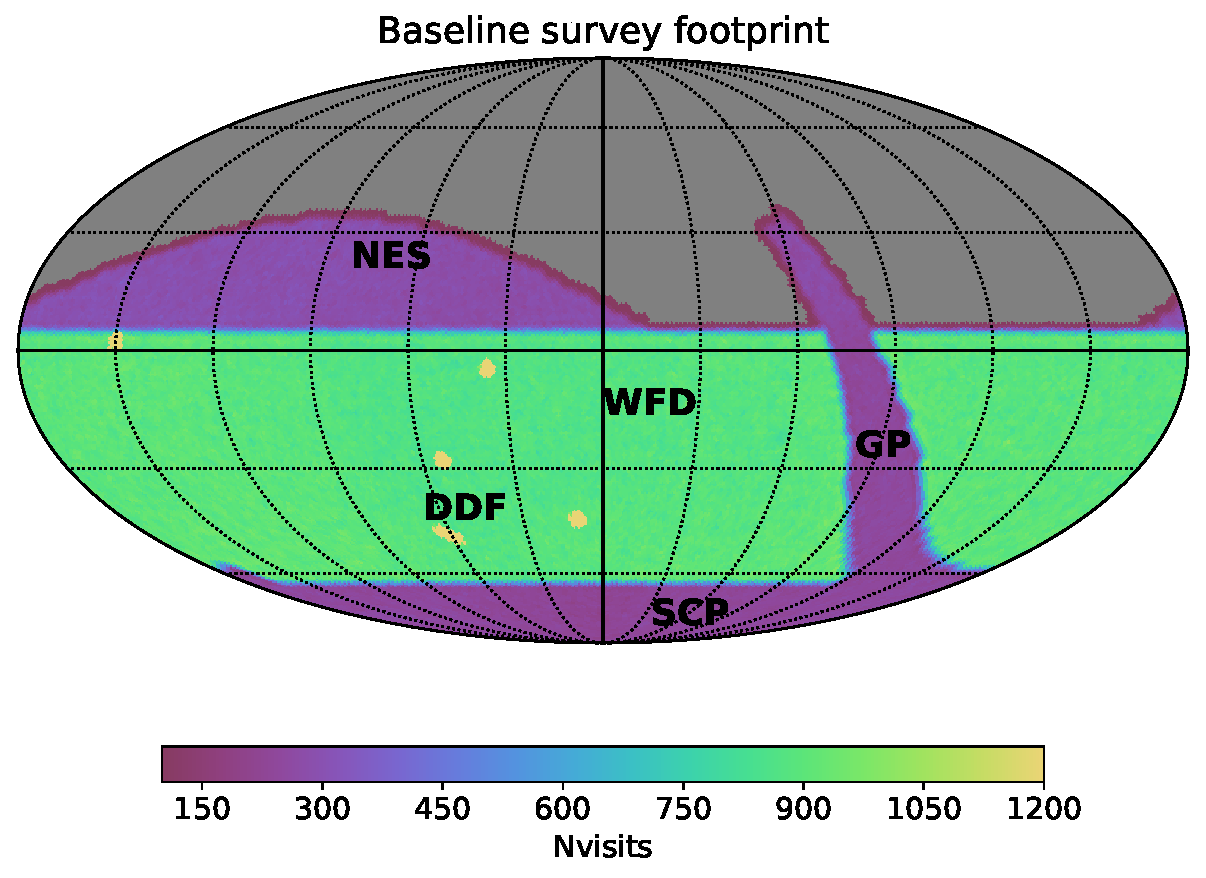
\includegraphics[width=0.65\linewidth]{graphics/Fink_Rubin_LSST/baseline_nexp2_v171_10yrs_nvisits.pdf}
    \caption{The baseline number of visits that Rubin will make across the Southern Sky. Taken from \textcite{bianco_optimization_2022}, the different areas on the map show the main survey, WFD, and additional mini surveys. With NES being the North Ecliptic Spur, DDF represents the Deep Drilling Fields, GP is the Galactic Plane and SCP is the South Celestial Pole. It is easy to see that different surveys using the Rubin Observatory require different viewing cadences to enable the collection of data that is desired.}
    \label{fig: Map of the fields that Rubin will visit with the median number of revists across different portions of the Southern Sky.}
\end{figure}

Over the course of the survey the expected number of alerts generated each night will be 10 million per night and within 60 seconds, transients will be reported \parencite{moller_fink_2021}. Of these alerts it is expected that there will be $\approx 1100$ SNe per night. This should enable the opportunity to discover more SNe Ia which will increase the odds of finding the EEx SNe Ia and could enable the beginnings of a population study with respect to their host galaxy properties. 

To handle this number of alerts, we employ the use of the Fink broker which allows for the processing of the large number of alerts from the alert stream of Rubin. Fink does the ingestion of the data of the LSST alert stream, annotation of the alerts such as early light curve classification and is capable of customisable filtering of the alerts \parencite{moller_fink_2021}. 

Fink employs machine learning methods of classification to disentangle the types of SNe that will be discovered by Rubin. These machine learning classifiers use an active learning approach that can take a smaller sample of training data and continually retrain the classification models to improve the models as the survey progresses in time\parencite{leoni_fink_2022}. This means that SNe Ia will be readily classified from the LSST alert stream producing science-ready images in mere minutes. 

\section{Project Aims} \label{sec: Project Aims}
Here we simply state the aims of the project, 
\begin{itemize}
    \item Curate a sample of Extra-galactic transients through Fink.
    \item Use the Fink broker to identify the Sn Ia in those transients using spectroscopic follow-up and machine learning algorithms.
    \item Use SALT3 to measure SN Ia properties \(c\) and \(x_1\)
    \item With a large enough sample, find EEx SNe Ia using the method laid out in \textcite{deckers_constraining_2022}
    \item Find correlations of EEx SNe Ia with DLR, host galaxy mass, global colour and SFR.
\end{itemize}

\section{Planned Methodology} \label{sec: Planned Methodology}
The proposed method for this project will be to ingest data from Fink, filtering the incoming data based on the scores that classification algorithms such as Early SN Ia, CATS and SuperNNova give to build an initial sample of SNe. Following on from that initial sample the method of \textcite{deckers_constraining_2022}. \textcite{deckers_constraining_2022} made cuts based on colour parameters derived from the application of the SALT2 model, where SNe Ia with \(-0.3 \leq c \leq 0.3\) are cut from the sample. Cuts are then made based on the stretch parameter \(-3.0\leq x_1\leq 3.0\), then a cut based on the peak magnitude in the g band of the observation \(-19.95\leq peak_g\leq-18.35\) and finally the first detection of the SNe Ia needs to be 14 days before the peak in the green bands luminosity was reached. \textcite{deckers_constraining_2022} argues that this is to remove peculiar SNe Ia from the data set and leaves only 'normal' SNe Ia in the dataset for analysis. 

It is unclear whether \textcite{deckers_constraining_2022} uses the following method for detection of EEx SNe Ia on the original starting sample of 127 SNe Ia or if it is on the sample of 115 SNe Ia post quality cuts. It is a reasonable assumption that the detection of EEx SNe Ia was done on the sample post quality cuts. 

The method to detect the EEx SNe Ia used in \textcite{deckers_constraining_2022} assess residuals in the light curves in flux space that are found by taking the difference between the best fit model light curve from the SALT2 model and the observed light curve. Specifically focusing on the span of time 6 days after the estimated explosion epoch which is determined from the best fit model. Although for this project, the SALT3 light curve model will be used due to its improved performance in the UV and blue wavelengths when compared to the SALT2 model. This is because these bumps, as mentioned in chapter \ref{sec: Supernova Ia physics and Progenitor Channels} subsection \ref{subsec: Early Flux Excess}, are universally near UV to blue throughout the excess.

Following the identification and classification of the EEx SNe Ia, the assigning of host galaxies will be done using the Directional Light Radius method, following this assignment the correlations of the EEx SNe Ia population in the sample with the properties of the host galaxies will be determined. These properties include but are not limited to the sSFR, stellar mass of the galaxy and the global colour of the galaxy. The colour of the EEx SNe Ia will also be a part of these correlative analyses to determine any correlations with host galaxy properties and the colour of the EEx SNe Ia. 

\newpage
\section{References} \label{References}
\printbibliography

\end{document}